\documentclass[10pt,twocolumn,letterpaper]{article}
\usepackage{cvpr}
\usepackage{graphicx}
\usepackage{caption}
\captionsetup{font=small}
\title{Figure candidates at CVPR print size}
\author{Preview for the authors (not manuscript text)}
\begin{document}
\maketitle
\begin{figure}[t]
\centering
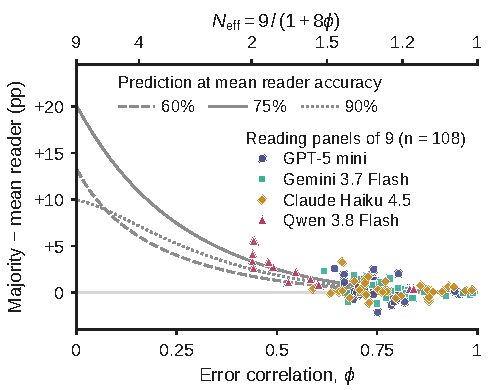
\includegraphics[width=\columnwidth]{fig1_teaser_col.pdf}
\caption{Candidate T-A (teaser, one column, 83.3\,mm). Majority minus mean reader accuracy against the readers' error correlation $\phi$ for all 108 nine-reader panels on yes/no items; curves, beta-binomial prediction at mean reader accuracy 60\%, 75\%, 90\%; top axis, $N_{\mathrm{eff}}=9/(1+8\phi)$.}
\end{figure}
\begin{figure}[t]
\centering
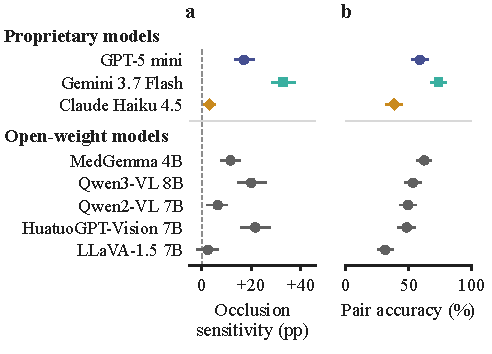
\includegraphics[width=\columnwidth]{fig5_region.pdf}
\caption{Candidate Fig.~5 (one column). (a) SLAKE-target: target minus control occlusion flip rate. (b) SLAKE-pairs: both answers of a pair correct.}
\end{figure}
\begin{figure*}[t]
\centering
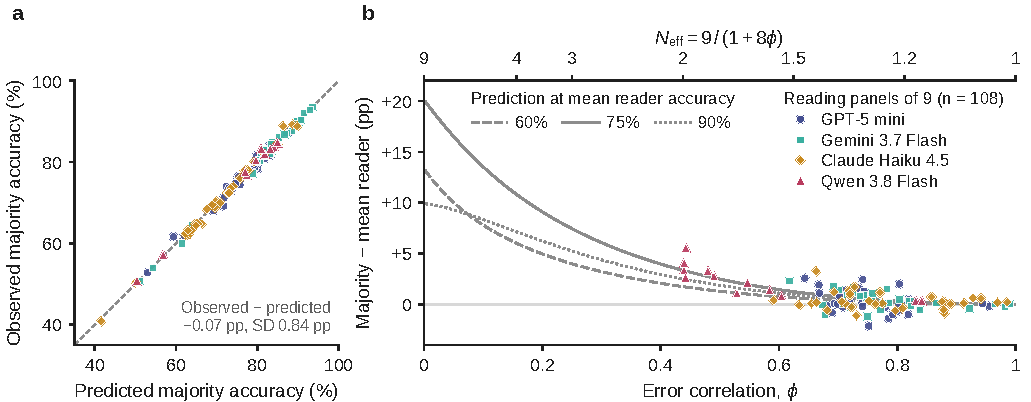
\includegraphics[width=\textwidth]{fig1_teaser_full.pdf}
\caption{Candidate T-B (teaser, full width, 174.6\,mm). (a) Observed against beta-binomial predicted majority accuracy. (b) As T-A.}
\end{figure*}
\begin{figure*}[t]
\centering
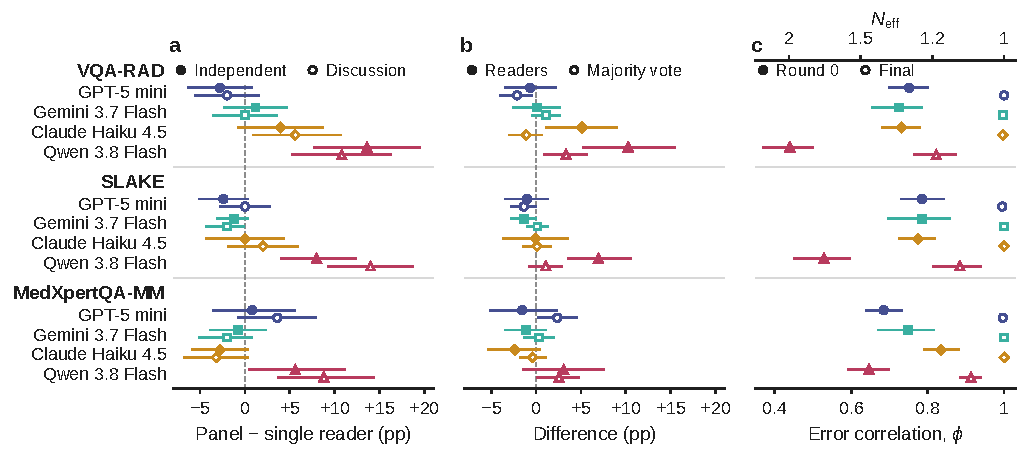
\includegraphics[width=\textwidth]{fig3_panels.pdf}
\caption{Candidate Fig.~3 (full width). (a) Independent and discussion panels of 9 minus the single reader. (b) The independent-panel difference split into mean panel reader minus single reader (Readers) and majority minus mean panel reader (Majority vote). (c) $\phi$ in round 0 and after discussion; top axis $N_{\mathrm{eff}}$.}
\end{figure*}
\begin{figure*}[t]
\centering
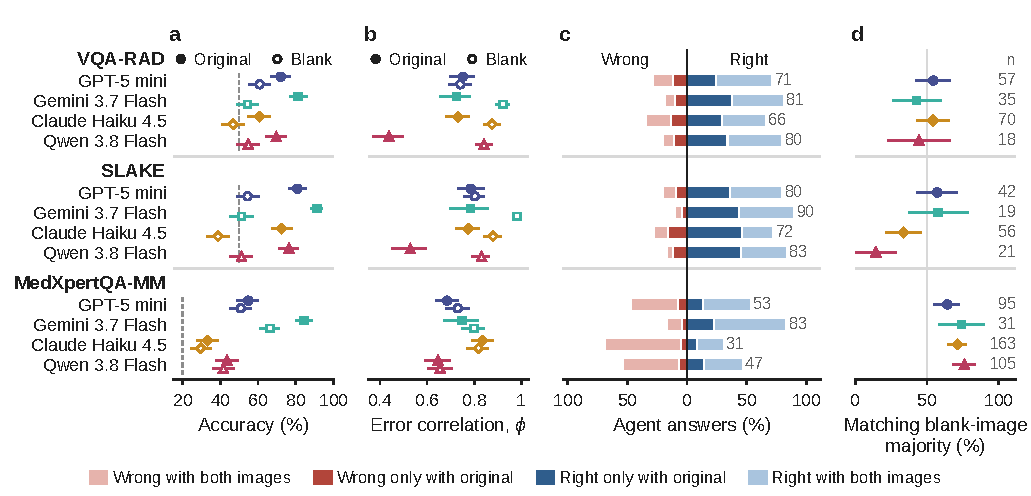
\includegraphics[width=\textwidth]{fig4_prior.pdf}
\caption{Candidate Fig.~4 (full width). (a) Single-reader accuracy with the original and the gray image; dashed, chance. (b) $\phi$ with each image. (c) Reader answers cross-tabulated by correctness with the original and the gray image. (d) Consensus errors whose majority answer is the gray-image majority answer; $n$, consensus errors.}
\end{figure*}
\begin{figure*}[t]
\centering
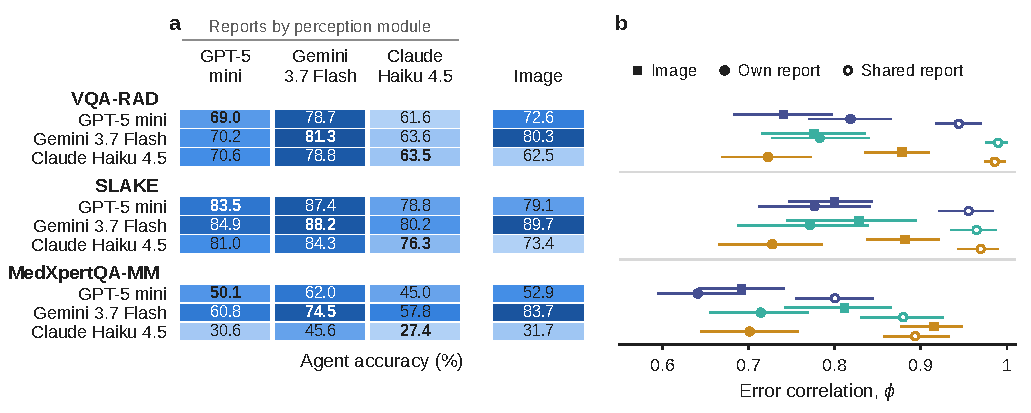
\includegraphics[width=\textwidth]{fig6_report.pdf}
\caption{Candidate Fig.~6 (full width). (a) Mean reader accuracy when each reader reads its own question-blind findings report from the column's perceiver, or the image. (b) $\phi$ of the 9 readers: image, own report, shared report.}
\end{figure*}
\begin{figure}[t]
\centering
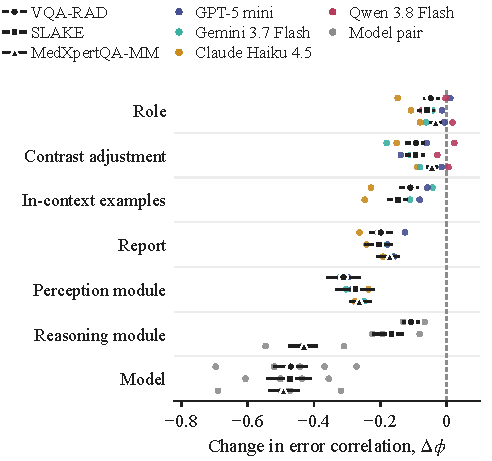
\includegraphics[width=\columnwidth]{fig7_contrasts.pdf}
\caption{Candidate Fig.~7 (one column). Change in $\phi$ when two readers of one model do not share the named component (matched within-model contrasts).}
\end{figure}
\begin{figure}[t]
\centering
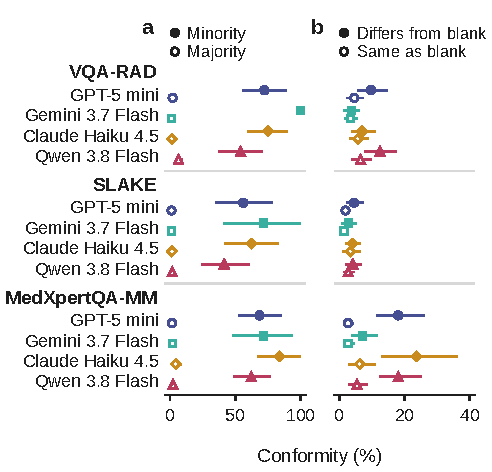
\includegraphics[width=\columnwidth]{fig8_discussion.pdf}
\caption{Candidate Fig.~8 (one column). Readers correct in round 0 and wrong after discussion, (a) by round-0 minority or majority, (b) by whether the round-0 answer differed from the same reader's gray-image answer.}
\end{figure}
\end{document}
